\chapter{绪论}\label{capater:intro}
轨迹大数据是移动互联网时代的产物,记录了移动对象的行为信息。通过轨迹数据分析技术可以挖掘人类活动规律与行为特征、城市车辆的移动模式、大气环境变化规律等信息。这些挖掘成果为研究城市发展、社会变迁和自然环境演变提供重要的参考价值。本文重点研究了轨迹大数据的管理和$k$近邻轨迹查询问题。本章中,章节~\ref{sec-c1-background}阐述了轨迹数据管理和$k$近邻轨迹查询的研究背景;章节~\ref{sec-c1-content}详述了本文的具体研究内容以及所遇到的挑战;章节~\ref{sec-c1-contribution}简述了本文的主要研究方法和研究贡献。

\section{研究背景}\label{sec-c1-background}
        随着卫星定位导航、无线通信和普适计算等高新技术的不断发展,带有定位功能的移动智能设备已被广泛应用,并成为社会生产、生活的重要组成部分。移动对象(含人、动物和车辆等)在主动或被动使用这些设备的同时,产生了大量记录其移动历史行为的轨迹大数据。例如:滴滴出行,全球最大的一站式多元化出行平台,在2017年10月发布的《第三季度全国重点城市交通出行报告》中称其每天新增的定位轨迹数据超过70TB\footnote{http://www.xiaojukeji.com/index/index}。轨迹大数据具有数据量大、数据增长快等特性。
            轨迹是地理空间在时间轴上形成的多维空间中的一条曲线,表示了移动对象在一段时间内时空信息等移动行为的变化。每条轨迹可看作一条时空采样点构成的序列,其中每个采样点记录了时间、位置、速度、方向等信息。
             从微观角度讲,轨迹数据蕴含了移动对象的移动模式与规律\cite{Gonz2008Understanding,Song2010Limits,LiDHKN10},例如从轨迹数据中我们可以发现市民的居住地、工作地和消费娱乐场所\cite{zzgSF}。从宏观角度来讲,海量的轨迹大数据蕴含了群体的移动迁徙和社会发展的变化,如城市的发展、交通的演化以及社会的变迁\cite{Zheng15}。通过轨迹分析等手段进行知识发现,并将它们运用在各种交通和服务应用系统中,包括交通导航\cite{QSJPredict,QSJProjection}、交通智能指挥\cite{LXX}、车辆异常监控\cite{CJY,MJLSoftware}、物流配送、城市规划、军事调度等\cite{QGD,XJJZXF,GQSurvery}。
        
         海量的轨迹数据具有重要的社会和应用价值,不仅为解决拥堵、改善交通服务、缓解能源紧缺和降低大气污染等社会问题提供了新的机遇,而且对认知人民的社会活动、优化公共资源配置、为建立新型共享经济有着特殊的意义。
       %  2017年12月8日,习近平总书记在中共中央政治局第二次集体学习时强调:实施国家大数据战略,加快建设数字中国。因此,轨迹大数据称为政府和企业的重要资源财富并得到广泛重视。
       %  在此背景下,轨迹大数据的分析和挖掘已经被学术界和工业界大量研究并成为数据挖掘领域的重要的新兴分支。
         在工业界,百度地图能根据实时轨迹数据进行路径规划。摩拜进行了基于自行车骑行目的地预测的研究\footnote{https://www.biendata.com/competition/mobike/}。美团和饿了么等外卖公司设计了基于轨迹数据的智能派单系统\footnote{http://blog.csdn.net/jinjin603/article/details/78793243}。上海电信根据手机信令数据研究了人口流动分析\cite{BT}。
         学术界业也出现一些针对轨迹数挖掘的热点研究工作,包括轨迹管理系统研究\cite{SharkDB,TanLN12,TrajSpark,trajectoryVLDB}
         查询可伸缩的快速轨迹聚类 \cite{DengHZHD15,CostaMM14,YuWWWH13,MaoSJZZ16}、轨迹流的连续查询\cite{NehmeR06}、路径规划及路径发现\cite{SacharidisPTKPMS08}、汇集模式发现\cite{ZhengZYS13}、旅伴模式发现\cite{TangZYHLHP12,LiCJT13}以及实时共享乘车\cite{DuanJWZY16}等。 
         
        
         轨迹相似性研究是轨迹挖掘和分析的核心内容之一。现有的轨迹数据间的相似性通常通过它们之间的距离来度量,即两条轨迹数据之间的距离越小,则认为它们之间越相似。根据这一准则,研究者们已经将广泛应用于时间序列分析的距离度量函数应用到轨迹数据中,这些度量准则包括:欧氏距离(Euclidean Distance, ED)\cite{DTKST}、动态时间弯曲(Dynamic Time Warping, DTW)\cite{bandwidth}、最长公共子序列(Longest Common Subsequence, LCSS)\cite{crowdsourced,SmartTrace}、
         实值序列上的编辑距离(Edit Distance on Real sequence,EDR)\cite{EDR}和 带有惩罚项的编辑距离(Edit Distance with Real Penalty, ERP)\cite{ERP}。
         此外,部分研究者针对轨迹数据特性设计了豪斯多夫距离(Hausdorff Distance ,HD)\cite{MaoSJZZ16}、弗雷歇距离(Fréchet Distance, FD)\cite{ZhuLYZHZ10,Guo2017}、一路距离(One Way Distance,OWD)\cite{LinS08}、带投影的编辑距离(Edit Distance with Projections, EDwP)\cite{RanuPTDR15}等。
         此外,还有部分学者针对轨迹的语义特性设计了用于计算轨迹语义相似度的距离\cite{Liu012,ZhaoX11,ZhengYZXSZ15}。尽管这些距离度量函数可以较好地捕捉到轨迹之间的相似度,但它们的计算复杂度高,要想应用到大规模轨迹数据集上需要进一步研究如何提高计算效率。
         此外,如何针对特定问题选择合适的相似度度量函数也是重要的研究内容\cite{Magdy2016Review,TooheyD15}。目前,仍然缺乏统一的查询处理框架以支持多种距离度量准则的应用。 
        
        本文主要研究了$k$近邻轨迹查询,即根据一条查询轨迹$\cal Q$找出$k$条与之距离最近(即最相似)的轨迹,是数据分析和挖掘的重要内容。其有着广泛的应用场景。比如说,交通部门想要开辟一条新的公交路线。其可以根据海量的人、车轨迹数据查看早/晚上下班高峰期间是否有$k$条与该路线相似的轨迹。此外,旅行平台可以通过查找某旅客的相似旅行轨迹给他推荐旅行伙伴或路线。此外该查询也有着广泛的科研价值,其是用户移动模式分析和异常轨迹检测等问题的核心内容。传统的集中式查询算法专注于查询时间效率的提高,常通过轨迹索引\cite{FrentzosGPT07,GutingBX10,KolliosGT99,RanuPTDR15,ChenSZZX10}、压缩\cite{AgrawalFS93,RafieiM02,Pelekis}和上、下界计算\cite{Skoumas,Zhao1997LINEAR}等方法来进行预剪枝从而避免过多的距离计算。  而海量的轨迹往往以分布式形式存储,即轨迹数据会分布在不同的数据节点上。因而已有的集中式算法无法满足分布式轨迹数据的查询需求。
        
            \begin{figure}
        	\centering
        	\subfigure[主从式]{
        		\label{fig:MS}   		
        		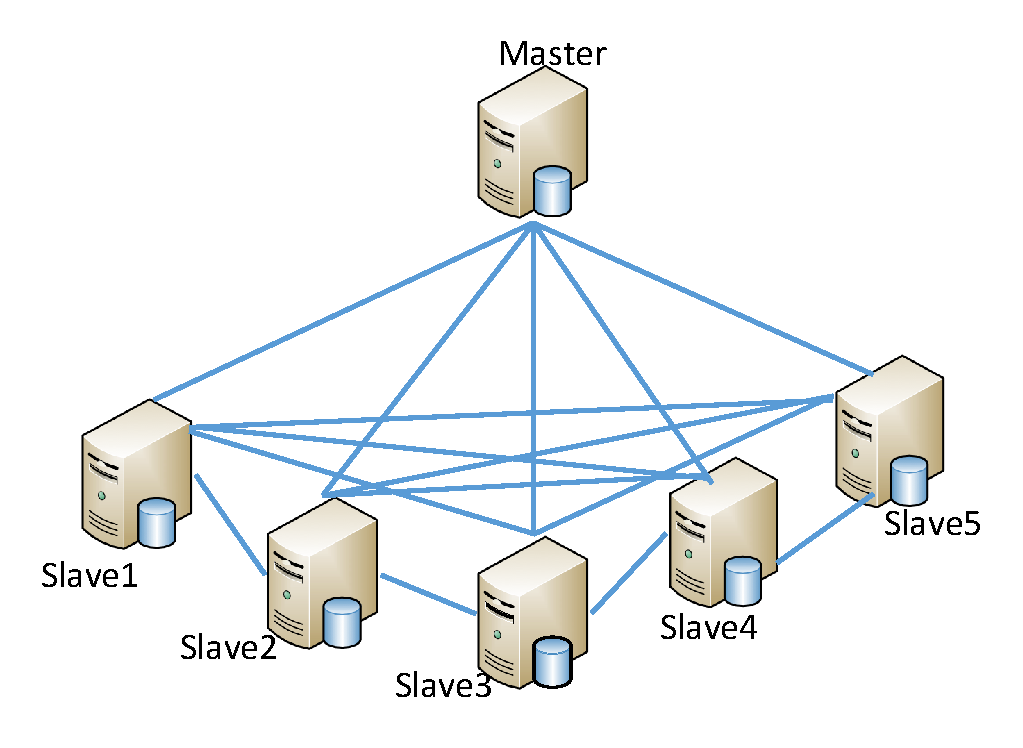
\includegraphics[width=2.7in]{Fig/chapter1/MasterSlave.eps}
        	}
			\subfigure[协调者-远程结点式]{
				\label{fig:CR}
				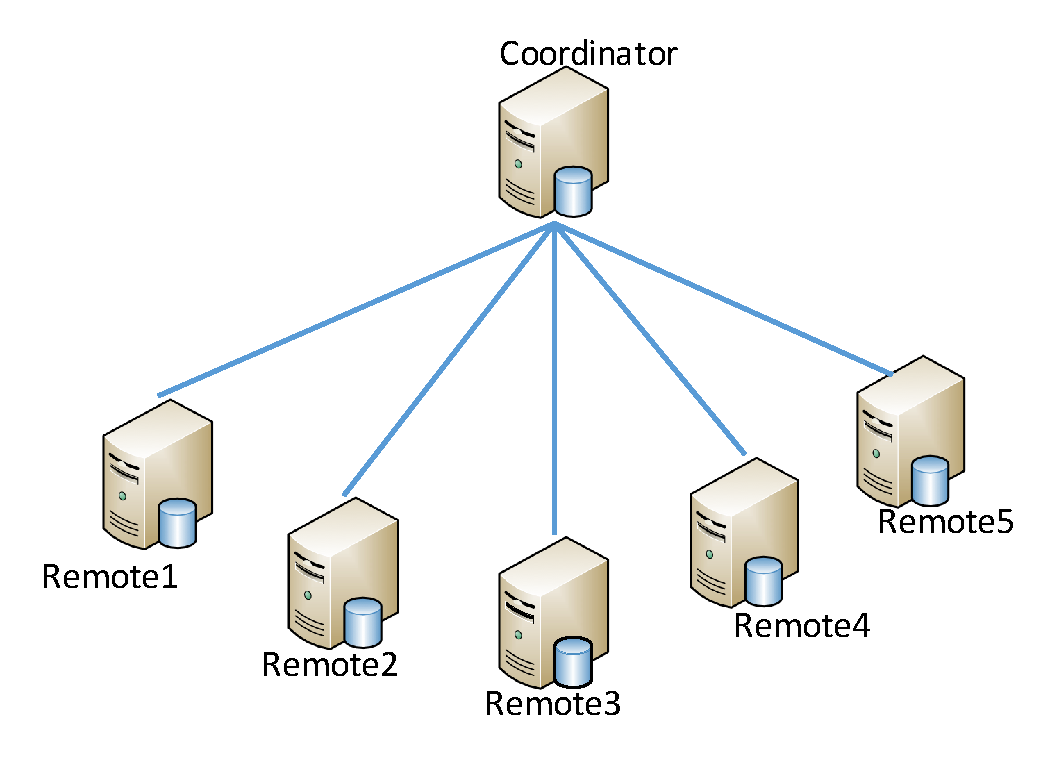
\includegraphics[width=2.7in]{Fig/chapter1/CoorRemote.eps}
			}
        	\caption{两种常见分布式架构}
        	\label{fig:DistributeArc}
        \end{figure}
        
        常用的分布式场景分为两种(如图\ref{fig:DistributeArc}所示):一种是基于主-从架构的。
        Hadoop和Spark系统就是典型基于主-从架构实现的系统,并随着这些系统的流行,该架构得到了广泛的应用。在主-从式中,系统包含一个主节点(Master)和多个从节点(Slave)。其中从结点存放具体数据并负责对本地任务的执行,主结点存放数据的元数据并负责任务的分发和调度。该架构往往要求所有物理结点在同一个集群内部,结点间通过高速网络连通。使用该框架进行轨迹处理分析的前提是,所有的轨迹都能被采集到一个数据中心中。在这种架构中,降低问题的计算开销是设计方法的首要考虑。
 另一种是  基于协调者(Coordinator)-远程结点(Remote)架构的。该架构中存在一个协调者和多个远程节点,其中协调者结点不存储任何数据只负责跟远程结点通信,而远程结点负责存放本地数据,且各远程结点间互不通信。 
 该架构一个典型应用就是众包(Crowdsourcing)。即个人或组织(协调者)将一个问题提交给一个群体(所有远程结点),
 群体中的各个单位,根据自身的知识来给出问题的结果。最终,提问者根据所有用户的答案获得最终结果。
 而在此架构中,降低问题的通信开销是解决问题的首要考虑。
        从图中,我们可以看出这两个架构的主要结构区别是后一种架构数据节点间彼此隔离互不通信,而第二种架构要求数据节点间能互相通信。这导致它们使用的应用场景也有所区别,第一种常用于集群内部,而第二种架构往往用于多个数据结点间构建连接。
        针对海量轨迹数据,   若都能被采集到某一数据中心(常见于滴滴等轨迹数据拥有者),则采用第一种架构进行管理。
        若由于采集、通信、隐私等原因,数据不能被统一存放到单一数据中心,往往以第一种架构进行管理。如每个智能手机拥有者,在各自的手机中保存了自己的轨迹数据,其他任何人都无法知晓其内容。针对这两种分布式场景,急需提出相应的$k$近邻查询方案。
        
        %特别地,相比于第二种方案,基于协调者-远程结点架构的查询算法还需要关注算法的通信开销。
        
        首先,使用主-从式架构进行$k$近邻查询前提是,我们已经采集了海量的轨迹数据并保存在集群中,且采集的数据集可能会不断增大。传统的轨迹数据库已无法满足需求\cite{BoteaMNS08,ChakkaEP03,Cudre-MaurouxWM10},而直接将海量轨迹以分布式文件(如HDFS)的方式存放在系统中,虽然简单、易行,但无法满足用户的查询分析的时效性需求。
        为此,我们首先需要对海量轨迹进行有效地管理以便提供低延时的查询结果。目前,已经有许多改造Hadoop、Spark等分布式系统,以构建满足轨迹数据的管理系统。这些系统根据存储介质的不同可分为两类,一类是基于磁盘的时空数据管理系统,典型的有TRUSTER\cite{MaYQZ09,YangMQZ09}、SpatialHaddop\cite{SpatialHadoop}、AQWA\cite{AlyMHAOEQ15}等。另一类是基于内存的管理系统,典型的有SpatialSpark\cite{SpatialSpark}、GeoSpark\cite{GeoSpark}、LocationSpark\cite{Locationspark}、Simba\cite{Simba}以及针对$k$近邻轨迹查询专门设计的TrajSimba\cite{trajectoryVLDB}等系统。已有基于磁盘的系统往往不能提供实时查询结果,而基于内存的管理不能满足数据不断增加的场景。为此,仍缺乏满足大数据要求的轨迹管理系统以提供低延时的查询结果。
        
        
        其次,在协调者-远程结点架构中,每个远程结点各自管理着本地的轨迹数据,且对于协调者和其他远程结点来说,其相当于一个黑盒,无法知道其保存数据的信息。
        而协调者结点扮演查询引擎的角色,其接受用户提交的查询,并将查询相关数据发送给远程结点。
        远程结点根据接收到的数据或请求,返回相应的查询结果或执行相应的操作。
        基于该架构的一种直观$k$近邻查询实现方法如下:协调者将接收到的查询轨迹直接发送给所有远程结点。远程结点根据接收到的查询轨迹,对其本地轨迹进行两两距离计算并将距离值返回给协调者结点。但该方案面临着通信开销过大的问题,其中通信开销值达到$O(n*M)$,其中$n$表示带查询轨迹的长度,$M$表示远程结点的数量。此外,由于该方案需要跟所有轨迹进行距离计算,从而导致时间开销也很高。为此,Smart Trace\cite{SmartTrace} 和 Smart Trace$^{+}$ \cite{crowdsourced} 等工作通过发送时间序列包围信封以计算最长公共子串距离上、下界并剪枝,从而降低计算开销。BandWidth\cite{bandwidth}通过多粒度包围信封计算动态时间弯曲距离的下界来逐步剪枝。
        LEEWAVE\cite{LeeWave}使用小波变换来降维时间序列数据并根据降维数据计算欧氏距离的上、下界来剪枝。以上优化都是针对一维时间序列数据,而轨迹数据是天然的多维数据。此外,它们都是针对某一具体距离度量方式进行针优化,优化方法不能迁移到其他距离下的查询中。为此,仍然缺乏通用查询方案。
                    

\section{研究内容与挑战}\label{sec-c1-content}
\begin{figure}
	\centering
	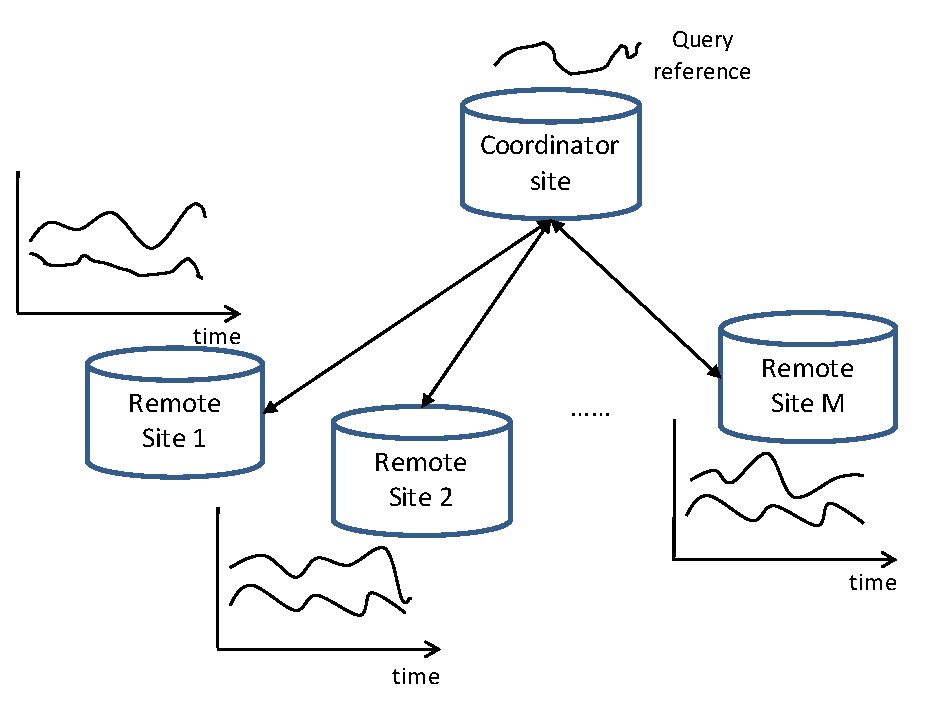
\includegraphics[width=0.73\textwidth]{Fig/chapter1/coor-remote}
	\caption{基于协调者-远程结点架构的查询展示}
	\label{fig-chapter1-demonstrate}
\end{figure}

本文针对海量的轨迹数据进行了分布式数据管理及分布式$k$近邻查询研究。首先,针对主-从式架构下的海量数据管理及查询,本文的研究目标是如何对获得的海量轨迹数据进行有效管理,并对以$k$近邻为代表的轨迹查询提供高效的查询接口。传统的集中式轨迹数据管理系统不能满足轨迹大数据的管理要求,而现有的基于集群的轨迹数据管理系统往往是基于磁盘的管理系统,存在着I/O开销较大的问题。
它们不能满足实时查询的需求,即用户给出查询轨迹后,需要在较短的时间内给出查询结果。目前,Spark等分布式计算平台因其良好的内存利用特性,成为提供实时数据分析的有效供给。本文的研究思路就是如何利用这些开源分布式内存平台,构建高效的轨迹数据管理系统。

其次,针对协调者-远程节点结构下的$k$近邻查询进行了研究。该结构下的轨迹数据管理如图\ref{fig-chapter1-demonstrate}所示,每个远程结点各自管理着
一批轨迹数据。协调者负责接收用户提交的查询和与远程结点进行通信。
在该框架中,协调者结点接收到用户的查询轨迹后,由于不知道各个远程结点中数据的任何信息。因此,一个简单的查询方案就是,协调者结点直接将查询轨迹直接发送给所有远程结点,并在远程结点计算查询轨迹与所有候选轨迹的距离。最后,协调者结点根据接收到的距离值,找出距离最近的$k$条轨迹。该方案简单易行,但由于需要将查询轨迹发送给所有远程结点,当查询轨迹数据量较大或远程结点较多时,存在着通信开销较大的问题。此外,由于需要计算查询轨迹与所有候选的距离,而距离计算往往复杂度较高。因此,该方案的计算开销也较大。为此,在该框架下,我们需要考虑如何设计出通信和计算开销都低的解决方案。

在处理$k$近邻查询时,还存在着一个不可忽略的问题即轨迹距离度量方法的选择。现有的轨迹查询和分析的工作往往都是针对某一选择或精心设计的度量方法以满足给定应用场景的需求。因此,现有的方法缺乏通用性。综上所述,

本文研究面临的挑战主要表现为以下四点:
\begin{itemize}
	\item \textbf{首先,针对获得的海量轨迹数据,缺乏高效的管理系统以提供低延时的查询结果。}基于集群的分布式数据管理方式,是处理轨迹大数据的必由之路。目前已经有许多基于分布式平台的轨迹数据管理方案,但这些方案大都是基于磁盘的管理系统,无法提供实时的查询结果。此外,这些系统大都是针对静态轨迹数据设计,不能满足轨迹数据不断增加的需求。为此,需要设计出满足能够对不断增长的轨迹大数据提供实时查询需求的管理系统。
	
	\item  \textbf{其次,针对时间序列上已有的$k$近邻轨迹查询技术往往只针对某一距离准则设计,缺乏通用性。}距离度量准则是轨迹数据挖掘分析的核心内容之一,选用不同的度量函数,导致的挖掘结果以及对结果的理解往往大不相同。现有的工作都是针对某一研究问题,精心挑选或自定义一距离函数以满足研究问题的需要。因此,所提出的解决方案具有较高的局限性,很难推广到其他的问题中。为此,需要提出通用或对一类问题适用的解决方案。
	
	\item \textbf{最后,现有协调者-远程结点架构下的$k$近邻查询面临着通信和计算开销过大的问题。}直接将原始查询轨迹发送到所有远程结点的方式,其通信开销随轨迹长度和远程结点的个数的增加而快速增大。而现有的数据降维方案虽然降低了数据的维度,但也造成了数据信息损失,使得数据不再直观且不能保证查询结果的准确性。此外,这些方法常用于处理一维时间序列数据,而轨迹是天然的多维时间序列数据。为此,需要提出新的轨迹数据降维方法,在保证查询结果正确性的同时,降低通信和计算开销。
	
\end{itemize}

\section{主要贡献}\label{sec-c1-contribution}
本文围绕分布式$k$近邻轨迹查询这一问题,系统性的提出了解决方案。首先,针对采集得到的轨迹大数据提出了基于主-从式架构的管理系统,该系统能对$k$近邻等查询提供低延时的查询结果。
接着,针对协调者-远程结点架构设计了两种通用查询处理策略,以解决通信开销过大和距离准则多的问题。这两个策略区别是第一种策略针对利用概要数据能同时计算距离上、下界的场景,第二种针对仅能利用概要数据设计出下界的场景。在这两种策略中,我们均使用多粒度概要数据来进行剪枝,并通过引入具体的度量准则验证了两个策略的有效性。
最后,使用真实轨迹数据集验证了算法的性能。因此,本文的主要贡献分为以下3点:
\begin{itemize}
	\item  \textbf{针对集群内海量轨迹数据的管理问题,设计了基于分布式内存的轨迹数据管理系统TrajSpark。}TrajSpark构建在分布式开源系统Spark之上,以充分利用分布式集群的内存资源并减少查询的I/O开销。
	为适应非结构化轨迹数据的管理需求,TrajSpark设计了适用于轨迹数据的表达方式IndexTRDD,并使用局部和全局索引相结合的轨迹索引策略此提供查询效率。此外,TrajSpark引入了时间衰减模型以适应轨迹数据不断增加所导致的数据划分开销较大问题。最后,针对三种典型轨迹查询设计了查询算法,并在真实海量轨迹数据集上验证了算法的性能。
	
	\item  \textbf{针对根据概要数据能同时设计出上、下界的距离函数,设计了同时使用上、下界针对协调者-远程结点架构下$k$近邻查询进行逐步剪枝的处理策略。基于该策略,实现了基于欧氏距离的查询算法。}协调者-远程结点架构下的$k$近邻查询的瓶颈在于通信和计算开销,本文使用降维技术以获取概要数据,并通过概要数据来进行距离估计并剪枝,从而达到降低数据通信开销的目的。针对根据概要数据能够同时计算出上、下界的场景,设计了使用多粒度数据逐步逼紧上、下界的剪枝策略。接着,针对欧氏距离,使用哈尔小波得到多粒度概要数据,并设计了适用于轨迹数据的距离上、下界。然后,将欧氏距离应用到我们所提策略中,设计了查询算法ED-FTB。
	最后,我们通过理论分析和大量实验验证了ED-FTB算法的有效性和可扩展性。
	
		\item  \textbf{针对根据概要数据仅能设计出下界的距离函数,设计了仅使用下界针对协调者-远程结点架构下$k$近邻查询进行逐步剪枝的处理策略。基于该策略,实现了基于动态时间弯曲距离的查询算法。}本文针对仅能根据概要数据计算出下界的场景,设计了使用多粒度数据进行逐步逼近距离下界和全局剪枝阈值的剪枝策略。接着,针对动态时间弯曲距离,设计了基于包围盒的多粒度概要数据,同时设计了适用于轨迹数据的距离下界。
		然后,将动态时间弯曲距离应用到该策略中,设计了查询算法DTW-FLB。
最后,我们通过大量实验验证了FLB-DTW算法的有效性和可扩展性。
	
	
%	\item  \textbf{针对通信开销较高问题,提出了两个通用查询实现框架FTB(Framework with Two Bounds)和FLB(Framework with Lower Bound)。}FTB框架中要求能根据降维后的概要数据计算出相似度距离的上、下界,并且需保证当细粒度的概要数据获取后,所计算出来的上、下界越来越紧并最终能收敛。FLB框架中仅要求能根据降维后的概要数据计算出相似度距离的下界,且仅需保证当细粒度的概要数据获取后,所计算出来的下界越来越紧。这两个框架由于仅需要传递查询轨迹的概要数据且仅需计算复杂度更低的界信息,因此能大大降低通信和计算开销。
%	
%	\item \textbf{针对FTB框架,提出了基于欧式距离的FTB-ED 算法。}为验证FTB框架的有效性,本文研究了如何将欧式距离嵌入到该框架中。为此,本文首先利用Haar小波变换以得到不同粒度的轨迹概要数据,并证明了全部概要数据的欧式距离等于原始轨迹数据的欧式距离。接着,利用部分概要数据,本文提出了针对欧式距离的轨迹相距离上、下界,并理论证明了界函数的正确性。然后,我们将该上、下界应用到FTB框架中,提出了FTB-ED算法。在该算法中,我们引入了性能优化策略以提高查询效率。
%	最后,我们通过理论分析和大量实验验证了FTB-ED算法的有效性和可扩展性。
%	
%	\item  \textbf{针对FLB框架,提出了基于动态时间弯曲距离的FLB-DTW算法。}为验证FLB框架的有效性,本文研究了如何将动态时间弯曲距离嵌入到该框架中。
%	为此,本文首先针对查询轨迹使用不同粒度的包围信封(Bounding Envelope)来表示轨迹的概要数据。接着提出了基于动态时间弯曲距离的下界,并理论证明了该下界的正确性。最后将该下界应用到FLB-DTW框架中,并提出了FLB-DTW算法。在该算法中我们引入了索引等多种机制以提高查询效率。最后,我们通过大量实验验证了FLB-DTW算法的有效性和可扩展性。
	
\end{itemize}


\section{章节安排}
\begin{figure}
	\centering
	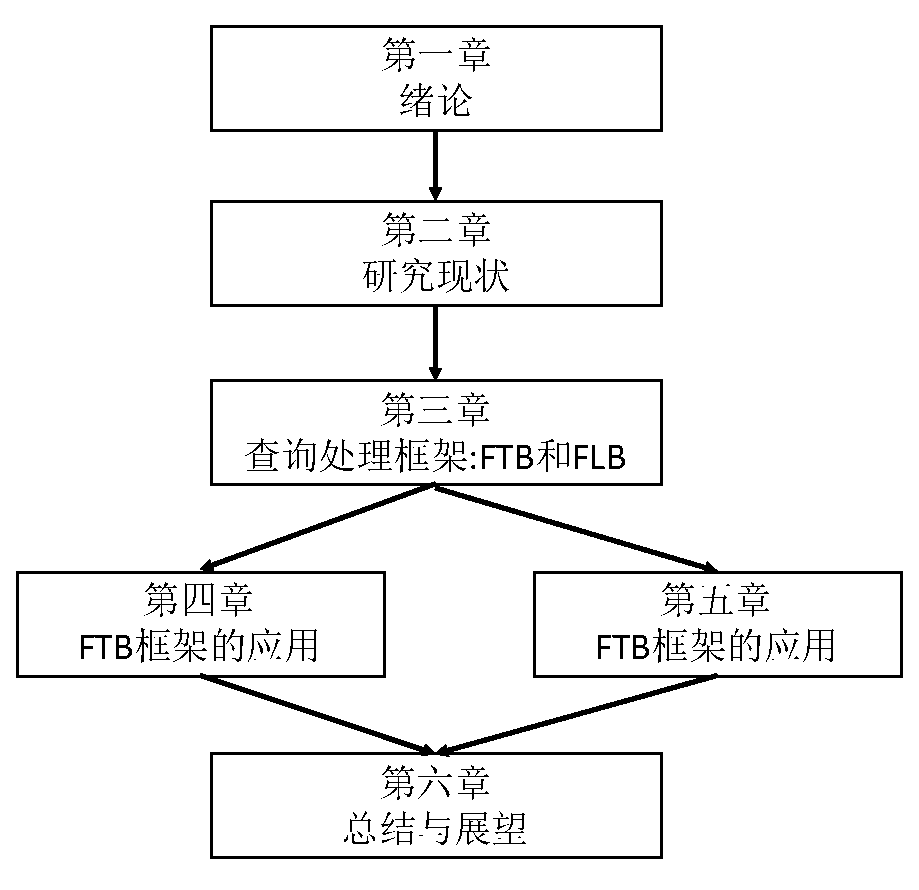
\includegraphics[width=0.73\textwidth]{Fig/chapter1/paperStructure}
	\caption{本文的组织结构}
	\label{fig-chapter1-structure}
\end{figure}
本文一共分为六章,章节安排如图~\ref{fig-chapter1-structure}所示:
\begin{itemize}
	\item 第二章从问题定义、轨迹数据管理、轨迹降维以及轨迹数据相似性查询三个方面介绍了研究背景知识和研究现状。
	\item 第三章介绍了基于集群分布式内存的轨迹管理系统TrajSpark,这一工作是基于主-从架构实现。
	\item 第四章介绍了使用距离上、下界并逐步剪枝的查询策略,并实现了基于欧氏距离的查询算法。
	\item 第五章介绍了仅使用距离下界进行逐步剪枝的查询策略,并实现了基于动态时间弯曲距离的查询算法。第四、五两章内容都是基于协调者-远程结点架构实现。
%	两个通用查询处理框架FTB和FLB以分别处理能同时提供上、下界的和仅能提供下界的距离准则函数。
%	\item 第四章介绍了如何将欧式距离嵌入到FTB框架中,并提供高效的查询结果。
%	\item 第五章介绍了如何将动态时间弯曲距离嵌入到FLB框架中,并提供高效的查询结果。
	\item 第六章对上述已有工作进行了总结,并展望了未来的研究方向和内容。
\end{itemize}

\clearpage
\phantom{s}
\clearpage